\documentclass{article}
\usepackage{multicol, caption}
\usepackage{graphicx}
\usepackage{geometry}
\usepackage{float}

\graphicspath{{./Images/}}
\geometry{
  a4paper,
  total={170mm,257mm}
}
\newenvironment{Figure}
  {\par\medskip\noindent\minipage{\linewidth}}
  {\endminipage\par\medskip}

% METADATA
\title{Comparing the Accuracy of the PRAISE-HK AQHI Modeling System to 
Real Measurements Taken with the PEK Sensors - Results and Personal 
Experience Report}
\author{Nolan Cheng}
\date{July 26, 2024}

% BEING DOCUMENT
\begin{document}
\maketitle
\begin{multicols}{2}

\begin{abstract}
  Over the span of roughly 6 weeks, I was tasked with utilizing the 
  Personal Exposure Kits, or PEK sensors, to compare the relative accuracy 
  of HKUST's PRAISE-HK model versus real measurements, in regards to the
  health risk associated with air quality. The major points of interest
  were not only how the PRAISE model deviated from real measurements, 
  but also how different microenvironments affected this deviation.
  I attempted to create and follow procedures in order to gather 
  data, and created software using Python to display, manipulate, and 
  compare this data. In the end, my results were not numerical as I had 
  hoped, but this was due to a lack of inexperience, knowledge, and time.
  I hope that my software and experience however at least reinforces 
  what should and should not be done in the future, even if not used
  directly.
\end{abstract}


\section{Concepts}
\label{section:Concepts}

The PRAISE-HK application records the users positional location, as well as 
the concentrations of various substances, including NO2, O3, SO2, PM10, and PM2.5.
PM10 refers to particulate matter below the size of 10 micrometers in diameter. 
Similarly PM2.5 refers to particulate matter below the size of 2.5 micrometers in 
diameter.

Important terms:
\begin{itemize}
  \item Diary: A representation of the daily agenda of different demographics of 
  people. It is what people of these groups are statistically most likely to be doing 
  during any given part of a day.
  \item AR\% (Added Risk): A measurement of the total inccured risk or risk factor that a single 
  element has on a persons health. The higher the percentage, the greater the risk.
  \item Exposure: The area under an AR\% graph versus time.
  \item IR (Infiltration Rate): A coefficient that measures the relative impact that 
  different microenvironments has on the AR\% of any given element. This is useful as 
  the PRAISE modeling system makes predictions based on what it thinks the outdoor 
  concentrations of elements will be, but this is clearly inaccurate if the user is 
  indoors. As such the IR coefficient helps to remedy this by lowering the AR\% by 
  some factor, bringing it closer to the actual value.
  \item Regression Coefficient: The relative danger of different substances, where 
  a higher coefficient means that the substance is more dangerous relative to other 
  substances.
  \item AQHI (Air Quality Health Index): A standardized method of determining the 
  genreal quality of the air in a region. AQHI values of 1-3 are considered low risk, 
  4-6 indicates moderate risk, 7-10 indicates high risk, and anything higher indicates 
  very high and serious health risks. This is just one of many standardized methods of 
  classifying air quality.
\end{itemize}


\section{Gathering Data}
\label{section:Procedure}

The first step was to ensure that the PEKs are calibrated and their 
measurements are reliable. I did not do this step however as not only 
does the process itself take quite some time, but learning how to do 
it myself would have taken even longer. As such, after being in touch with 
Dr Ning and Comet, I had 4 PEKs calibrated.

The next step was determining the best method of gathering 
measurements from the PEKs so that the data could be parsed later. 
This would be done first by taking a minimum of two PEKs to various locations 
around Hong Kong so as to reduce experimental uncertainty. Following the advice of 
Alexis, I created itineraries for the days that I planned to take measurements,
and based my itineraries off of diaries 
so as to emulate the microenvironments that various people were 
exposed to on a daily basis. I created my itineraries using Google's
"My Maps" feature found at https://www.google.com/maps/d/u/0/, which is
noteably not the exact same as Google Maps, but a sub-feature of it. This 
is just the software that I decided to use to plan my trips, however 
there are plenty of free alternatives online as well as the option to use 
a physical map.

In total, I created only 2 itineraries due to having a limited amount of time 
here after being out sick with a cold for abuot 4 days. The first itinerary
I created resembled that of a person who worked as a homemaker 
(\ref{figure:DiaryHomemaker}), and the second 
itinerary I created resembled that of a retired person
(\ref{figure:DiaryRetired}).

Note that during this time, I was still partially sick and also alone in my 
travels so did not feel comfortable going to places I did not really know, and did
not want to stay outside too long. This is why the two itineraries I created 
were in the same locations, and I did not do an itinerary that involved me 
being outdoors for a long period of time. I did however take measurements on a third 
day, but did not follow an itnierary that I had created.

\begin{figure}[H]
  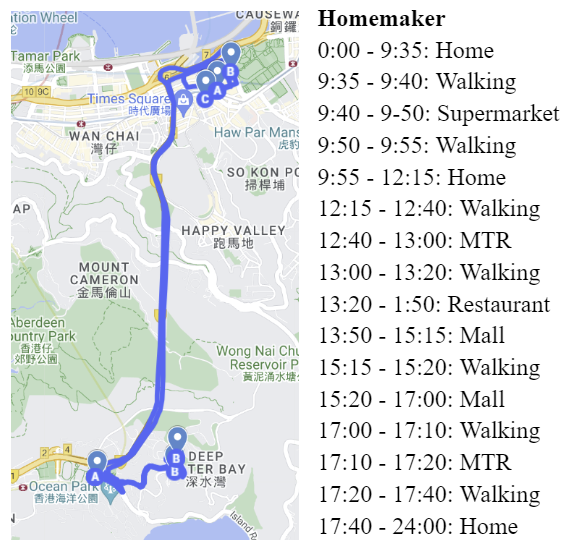
\includegraphics[width=\linewidth]{Diary_Homemaker.png}
  \caption{\label{figure:DiaryHomemaker}Homemaker Diary}
\end{figure}

\begin{figure}[H]
  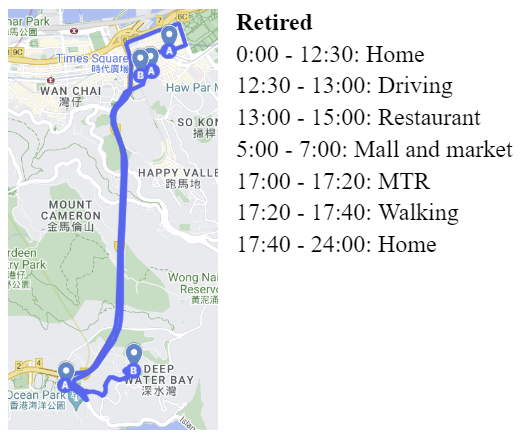
\includegraphics[width=\linewidth]{Diary_Retired.png}
  \caption{\label{figure:DiaryRetired}Retired Diary}
\end{figure}

While out on the paths of these diaries, I took only 2 of the 4 PEKs that I had access to.
This was primarily because carrying more than two PEKs on my person was not easy, as I 
did not have a steadfast mount for them, but instead they were hanging, leading to them being
susceptible to hitting into things as I walked.

After each day, I would take the PEKs back to my house and place them next to each 
other in my room. This would allow me to see how far the two had varied from 
each other, and compensate in my analysis later if necessary, as the PEKs never 
stayed perfectly calibrated.

Once I completed the diaries, I created a program that generally parsed the data I collected, 
analyzed and manipulated it, and then displayed it. One aspect of this analyzation, would be
converting the collected data from the PEKs, which was only concentration data, and 
turning it into the AR\% values that we would be comaparing from the PRAISE model.
This can be done by the following equation, 
$IR \times (e^{\beta \times C} - 1)$
where IR is the infiltration rate for that substance, $\beta$ is the regression coefficient,
C is the rolling average (over 3 hours by default), and e is just the constant e.
Besides the backend data analysis and manipulation, 
this program would provide primarily a visual representation of the data being analyzed.


\section{Software}
\label{section:Software}

Starting my experience here, I had used python an intermediate amount before in order 
to learn basic programming for making small tools, as well as learning how to create
neural networks, noteably with the PyTorch library. During my time here however, I expanded
my knowledge and experience greatly.

I began by learning to utilize a library called Selenium, which allowed me to automatically 
parse the PEK data from the online SEIN website without having to do this manually each
time. The program works by emulating a browser as if a human were using it, allowing me
to navigate the SEIN website, including the login page. While I'm sure that there are 
multiple ways, and likely better ways to accomplish this, this is the easiest method that 
I had found online doing limited research.

After being able to automatically parse the PEK data, I developed a program to display this 
data using the popular matplotlib library. It first not only unpacks the PEK data gathered 
from online, but also data from the PRAISE application of my position, as well as data from
the PRAISE servers detailing my exposure at different places and times.

\begin{figure}[H]
  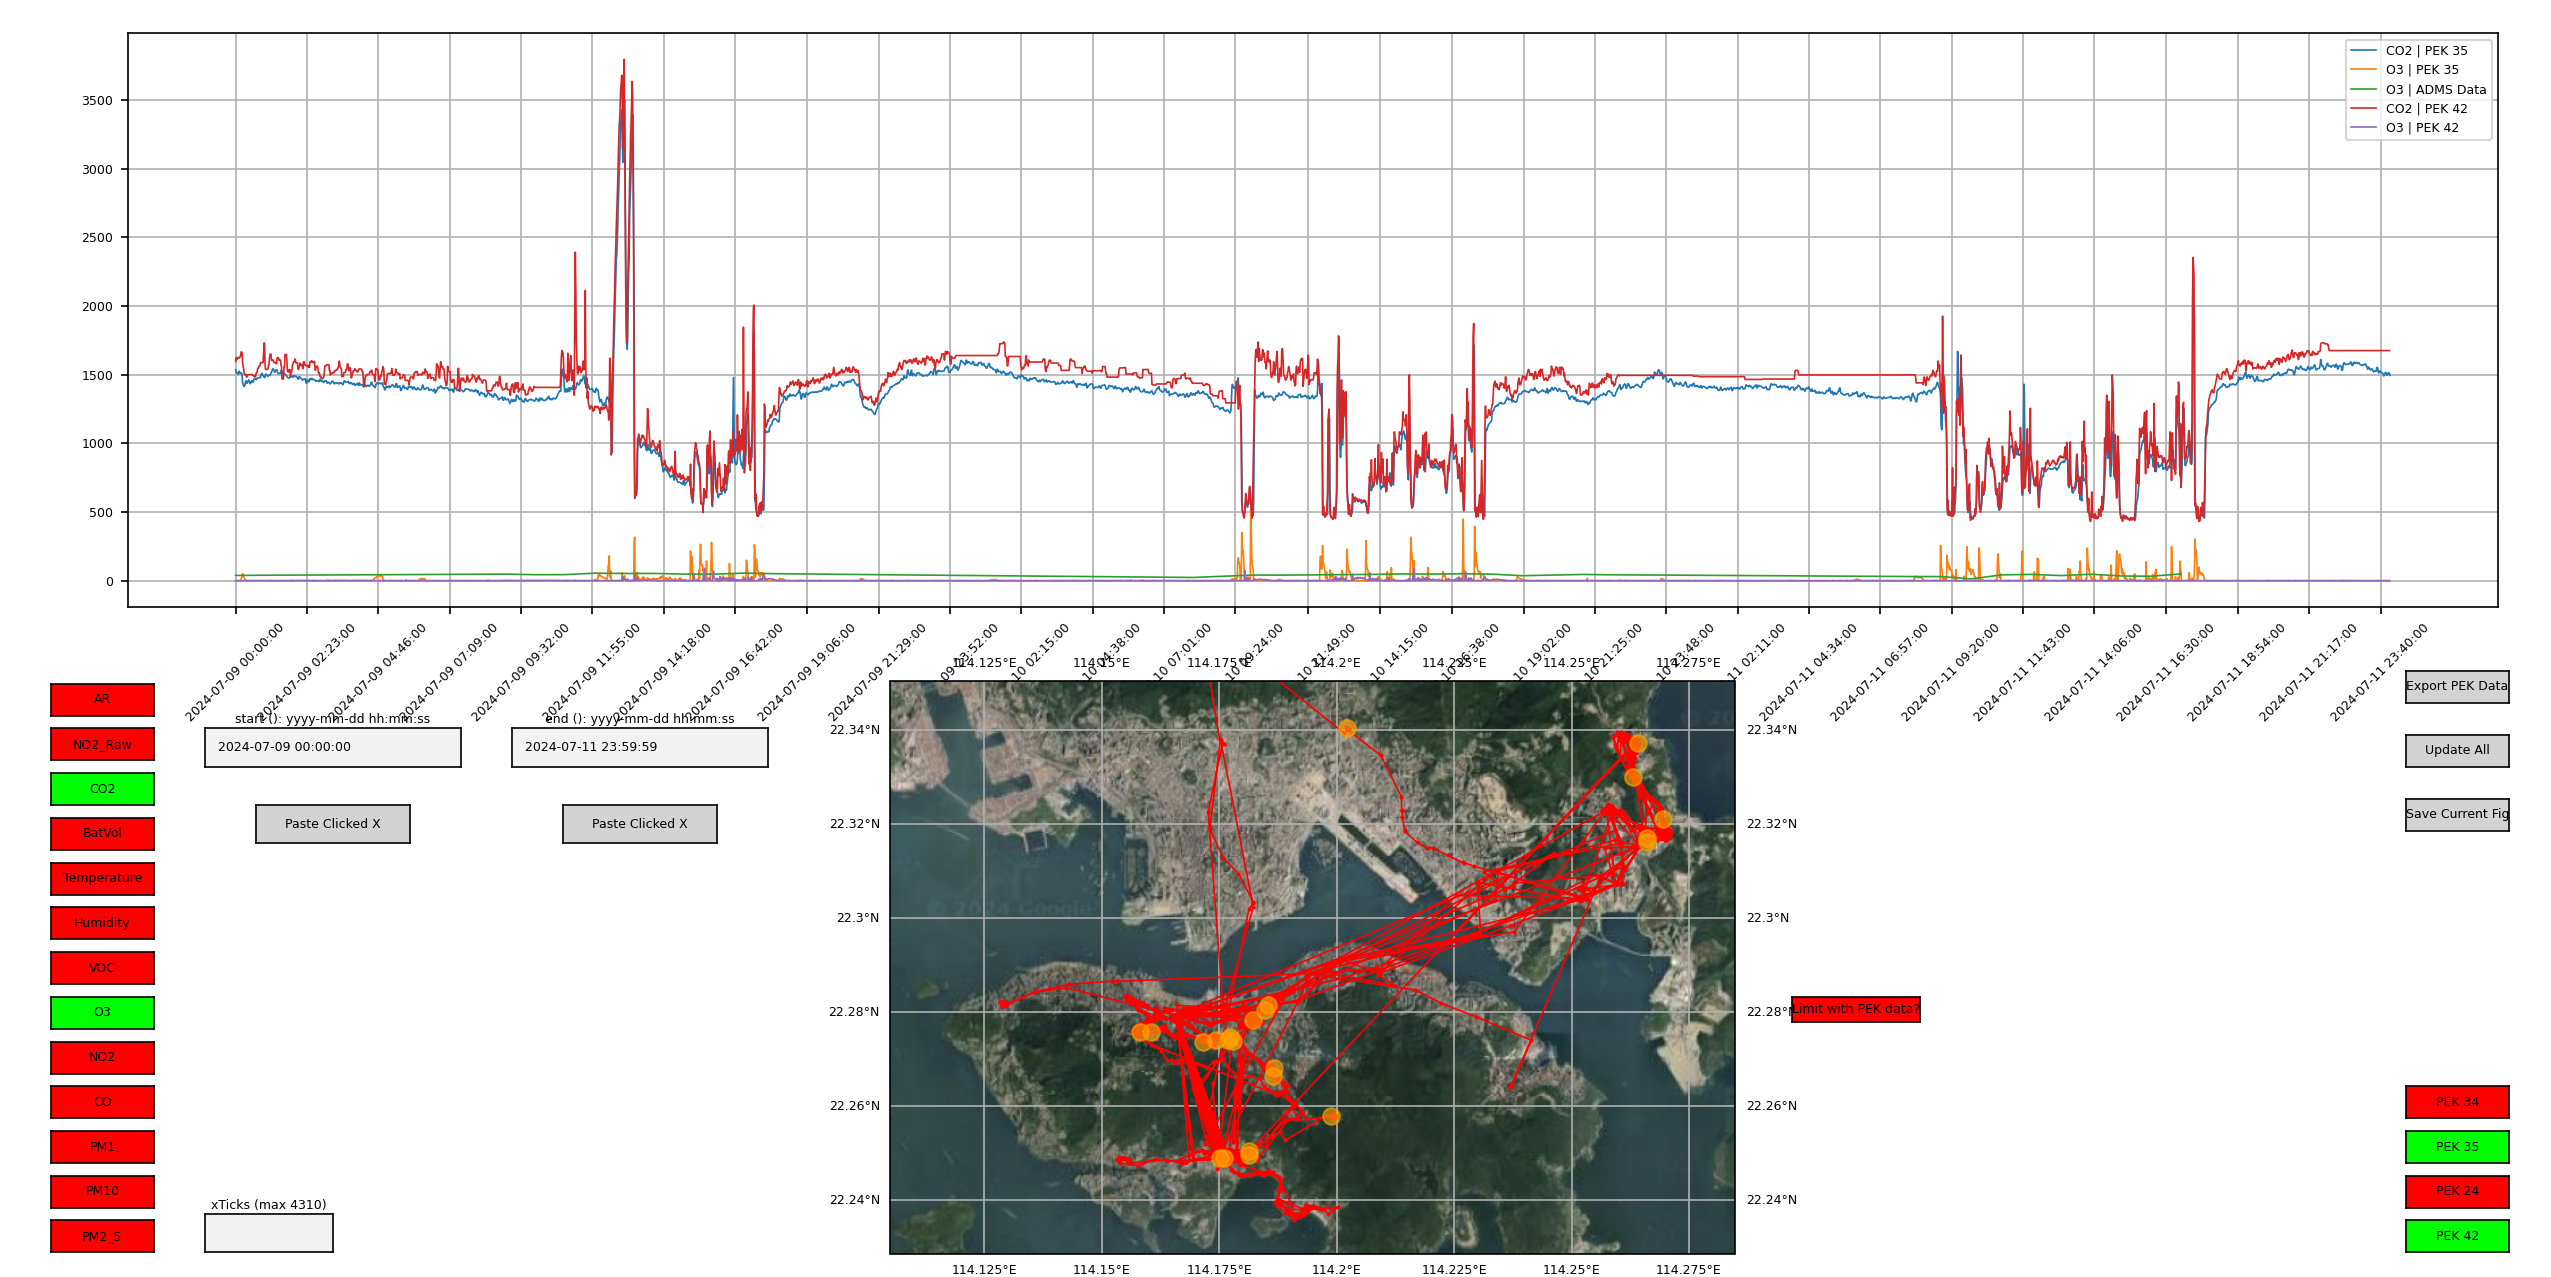
\includegraphics[width=\linewidth]{GUI_example_1.png}
  \caption{\label{figure:GUI_example_1} Example of the GUI I created}
\end{figure}

The program has two main plots, with one to display numerical data from the PEKs and PRAISE,
and the other showing the positional data of where I'd been from PRAISE (what I refer to as 
the data and map subplots respectively). Note the map subplot has a satellite image overlayed
on top of it, but this image must be manually updated if a larger image is needed.
It includes various miscellaneous functions, including:
\begin{enumerate}
  \item \label{item:PEK_element_buttons} Dynamicly created buttons to toggle what PEKs and what numerical values you 
  want to have displayed (dyanmically referring to buttons not being hard coded but
  instead that react to which PEKs are automatically pulled from the SIEN website, 
  and what type of data is available on each as some have more types of data than
  others). These are shown to the right and left of the screen under the data
  subplot, and are in red andgreen to indicate them being toggled visible or not visible.
  \item \label{item:limiting_textboxes_buttons} Text boxes and buttons to limit the numerical data shown based on time intervals.
  These are shown directly to the right of the toggleable buttons (\ref{item:PEK_element_buttons})
  on the left of the screen.
  \item \label{item:xticks_textbox} A text box that allows the user to change how many tick marks appear on the data 
  subplot, allowing for higher or lower resolution parsing by time. This is shown in the very
  bottom left corner of the screen.
  \item \label{item:SEIN_export_button} A button to automatically export the PEK data from the 
  SIEN website. This is on the right of the screen beneath the data subplot.
  \item \label{item:update_all_button} A button to force update both the data and map
  subplot in the event that something goes wrong. This can be shown beneath the export data button
  (\ref{item:SEIN_export_button})
  \item \label{item:save_current_figure_button} A button to save an image of the current
  figure for later reference. This is shown beneath the update all button (\ref{item:update_all_button})
  \item \label{item:limit_graph_data_button} A toggleable button that allows the user to 
  switch between being shown all positional data parsed from PRAISE, and clipping this data
  to match the time frame on the data subplot. This button can be shown directly to the right 
  of the map subplot.
  \item \label{item:clicking_data_subplot_function} A general function that tracks where the 
  user clicks on the data subplot, allowing that date to be pasted into the time frame
  limiting textboxes (\ref{item:limiting_textboxes_buttons}), as well as casuing a light blue dot 
  to appear on the map subplot, indicating the closest PRAISE positional datapoint at that
  time. There is a vertical line that indicates where the user last clicked, as seen in 
  roughly the center of the data subplot.
\end{enumerate}

In addition to these interface functions, there are multiple algorithms to unpack, 
clean, and analyze data in a useful way that run on the codes initialization. This includes: 
\begin{enumerate}
  \item Unpacking the PEK, PRAISE, and PRAISE servers data.
  \item Turning two coordinates of latitude and longitude into the distance between them 
  (in kilometers).
  \item Logging most if not all errors, warnings, and general operations such as how
  long functions take to execute. This is primarily for debugging purposes and saves
  to a recentlogs file. No past logs are kept, and new logs are always overwritten (as 
  it is now, but this can be easily changed)
  \item Cleaning the PRAISE positional data, as some of it is messy or blatanly 
  wrong. This is primarily done by filtering outliers that indicate the user 
  moved at speeds exceeding roughly 108 km/h or moving in ways that indicate sharp 
  and drastic turns below 20 degrees between any 3 positional points.
  \item Using location variance to determine locations where the user was stationary 
  for a prolonged period of time. This can be seen in the map subplot indicated by 
  large semi transparent orange dots.
  \item Averaging PEK data to smooth rough curves (not highly effective).
  \item Matching PRAISE server exposure data to PEK data in order to generate 
  exposure and AR\% data that can be compared. 
  \item As the data from the PRAISE model gives the AR\%'s for multiple positions 
  at the same time, the program also sorts this data and only compares the AR\% data 
  for locations that the user actually visited
\end{enumerate}


\section{Results and Potential Improvements}
\label{section:Results}

By comparing the PRAISE server's AR\% data to the calculated AR\% I had calculated
from the PEK data, I was able to create the graph featured in Figure 
\ref{figure:AR_comparisons_1}.
\begin{figure*}[!tp]
  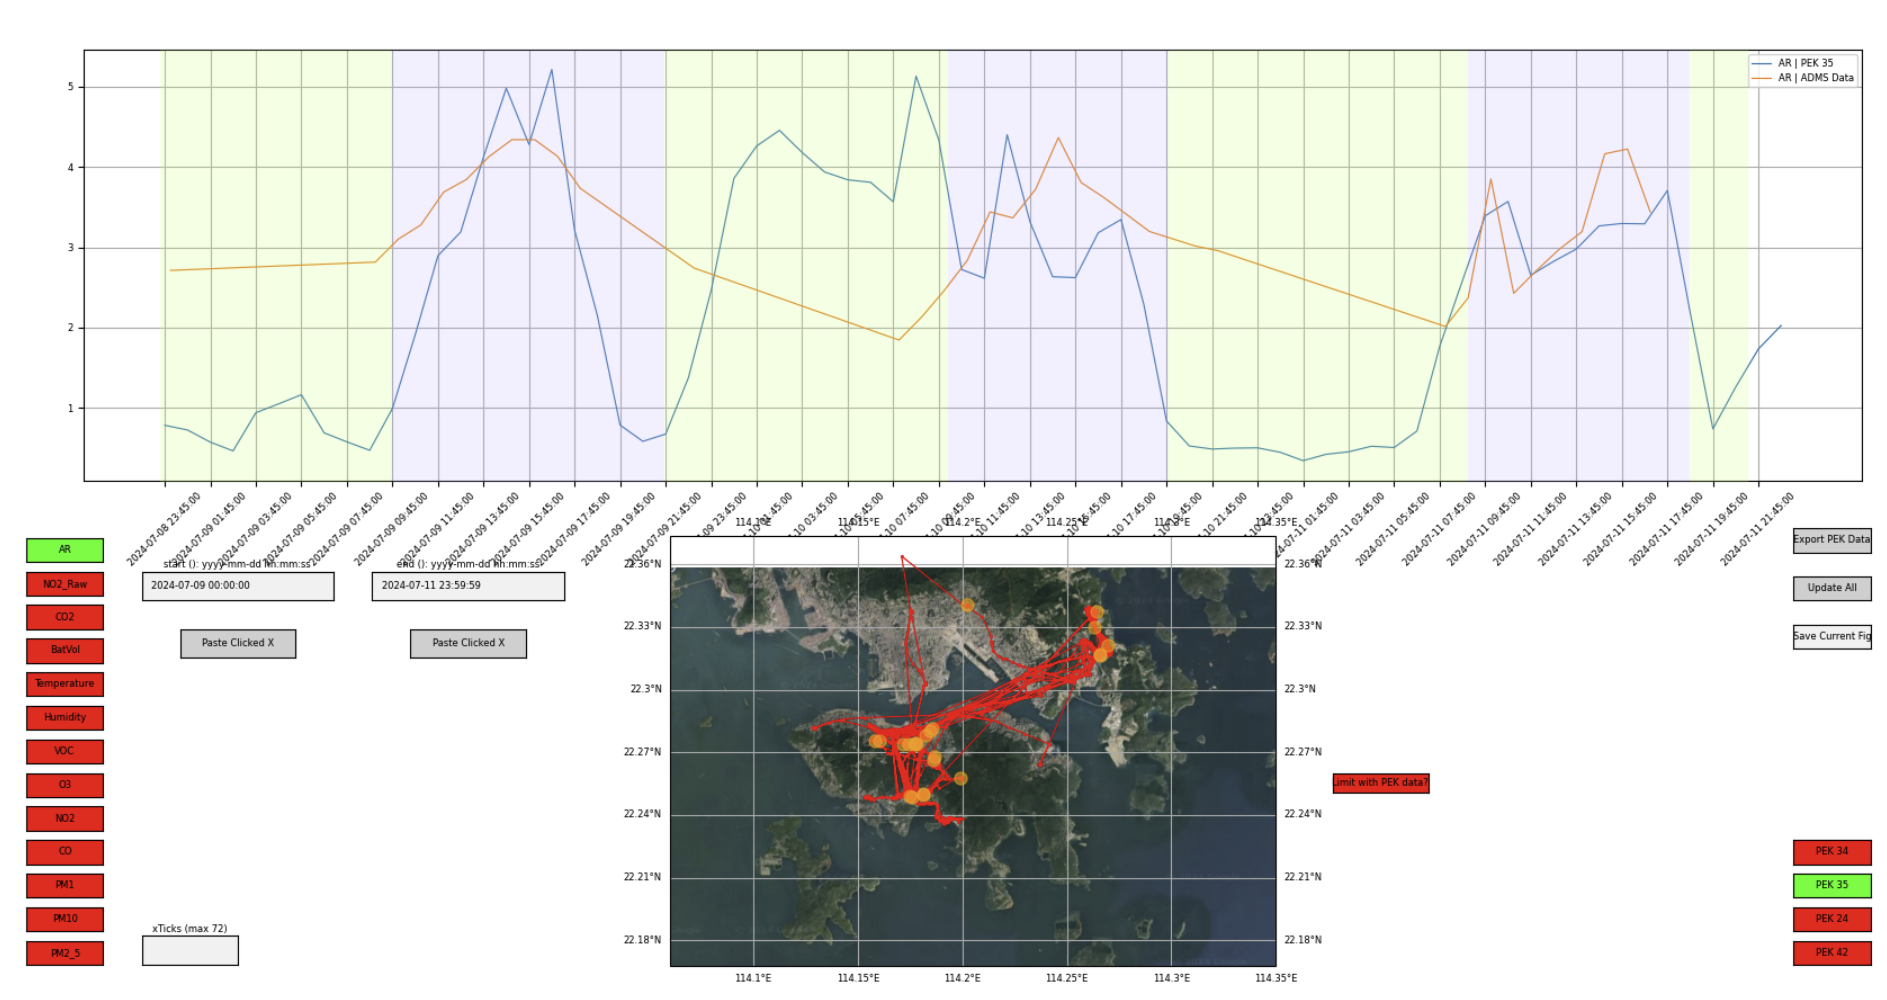
\includegraphics[width=\linewidth]{AR_comparisons_1.png}
  \caption{\label{figure:AR_comparisons_1}}
\end{figure*}

As we can see, during the day when I was completing diaries, the AR\% taken from 
the PRAISE model (as shown in orange) closely resembles that of the real measurements
(shown in blue), the times of which are highlighted in magenta. The measurements do vary
vastly at the beginning and end of these time frames, however this can be attributed to 
the fact that the AR\% are calculated on a 3 hour rolling average.

The green sections mark the period of time that I was at home and asleep, with a very
noticeable gap between the real values measured by the PEKs, and the predicted values 
by the model. The exception to this however, is in the second green region from the left, 
where apparently the AR\% in my room exceeded that of the models predictions. While I 
am relatively sure that the other green regions are so vastly incorrect is due to the fact 
that the infiltration rate coefficients I used were not completely accurate for the 
microenvironment that I was in, I am not certain as to why this second region from the 
left is so different. I assume it is due to either me forgetting to turn on air conditioning, 
or potentially placing the PEKs behind my computer fan which was going all night. This leads
me to the major places of improvment that I can think of in my procedure as well as software.

Due to my limited knowledge about data science, my limited time, and low experience, I was 
sloppy in a number of fields. Some of the most major improvments that I can think of are:
\begin{itemize}
  \item Creating a larger quanity and a larger variation of diaries. This larger and more 
  diverse dataset would allow for better data analysis and more opportunities 
  for understanding patterns in the data. As I went to the same location in both diaries 
  that I followed, and then wandered for the third day I recorded data, I do not know
  if the results I found were accurate on a larger scale or if they were just due to 
  the model being accurate in one location, but not others. 
  \item Following diaries more closely and actively recording the microenvironments I 
  was in. This would have greatly increased my technical understanding of why 
  certain time frames had the values and concentrations that they did, such as in the 
  highlighted green region, and why its calculated AR\% were so much higher than that of
  the other green regions.
  \item The way that I determine the infiltration rates of each element depends on my
  algorithm to locate regions of low variance 
  (shown in Figure \ref{figure:AR_comparisons_1}'s map subplot indicated by the semi
  transparent orange dots). The algorithm sets the infiltration rate to some nonzero 
  coefficient given to me by prof Jimmy if the users position at any given time is 
  within a certain distance threshold of these points of low variance, as I assume that
  these locations means the user is stationary. And as the majority of the time, if 
  a person is geographically stationary, they are more likely to be inside than outside.
  This logic however is clearly flawed, and more in depth analysis would need to be done 
  to not only calibrate the thresholds to determine the points of low variance, but whether 
  or not this location is indoors or outdoors.
  \item Adding onto the previous item, the way I determine points of low variance 
  is by calculating the variance between a certain number of individal points. In the future
  however it may be more accurate to calcuate the variance based on time chunks instead 
  of the number of points, as when a point is created varies widely from a few seconds or minutes, 
  up to a full hour, making variance calculation using this method not fully reliable.
\end{itemize}

In addition to places where I believe my procedure could be improved, some of the features 
that I thought about implementing but didn't have the time to include:
\begin{itemize}
  \item Using the python library geopy to reverse geocode latitudes and longitudes into 
  addresses and buildings. This process would help to fix the issue of determining whether
  or not a location of low variance is indoors or outdoors, as if a reverse geocoded 
  location is within the proximity of the low varaince location, it is safe to assume the 
  user is indoors, however if the reverse geocoded location is relatively far from 
  the location of low variance, it is more likely that the user is outdoors and stationary.
  This does however rely on a reliable method of determining locations of low variance, 
  which needs to be calibrated more finely.
  \item Adding textboxes and buttons to the GUI that allow for manually changing the 
  thresholds for various backend data analysis functions, including the one to determine 
  locations of low variance. As of now, the program only performs these calculations on 
  initialization. As each initialization could take up to 10 seconds however, it would be 
  much faster if these thresholds could be calibrated in the GUI itself instead of needing
  to reload the code every time.
  \item Adding the exposure calculations. I simply ran out of time to implement the 
  algorithm for calculating the exposure of individuals based on their AR\%'s. 
  \item Creating an algorithm to numerically determine how accurate the PRAISE system
  is at modeling various microenvironments. This is a mixture of not having a system to 
  accurately determine the users microenvironment in the first place, as well as not 
  understanding how one would go about doing this in the best way. I did not have enough 
  time to research this or discuss it with a professor.
\end{itemize}

\section{Closing Words}

As a whole I am not compeltely satisifed with my results as they are largely 
numerically unfounded, but am glad that I now 
have a much better foundation on how to conduct procedures in the future. I hope that my 
software is useable moving forward, however understand that it is not the best or 
most advanced system. Although I am departing from Hong Kong, I would love to get feedback
on specifically what I could have improved on.

\end{multicols}
\end{document}